\documentclass[10pt,final,journal]{IEEEtran}
\usepackage{graphicx}

\begin{document}
\title{Self-Partitioning Cloud Datastore for Scalable Transaction Processing Proposal}
\author{Benjamin Busjaeger, Jonathan Chu, Daniel Ormond \\
\{busjaeg2, jmchu2, ormond1\}@illinois.edu}
\date{Feb 2012}
\maketitle

\begin{abstract}
We are designing a new cloud data storage system that will be highly scalable and yet still be able to provide strong data consistency guarantees. Our system extends existing cloud key/value stores with modular components for transaction management and access-based partitioning. We plan to utilize graph theory, clustering algorithms, and Markov chaining to co-locate related data for efficient transaction processing and to assign partitions to optimal locations in the server clusters. Through continuous analysis of execution logs, our system should be able to recognize data access patterns and use that knowledge to partition data within the cluster to better fit within those patterns. With our data partitioning scheme, we hope to lower time delays, reduce bandwidth, and ultimately improve the speed of online transaction processing without sacrificing data consistency.
\end{abstract}

\begin{IEEEkeywords}
cloud, data storage, transaction processing, partitioning
\end{IEEEkeywords}

\section{Introduction}
Cloud Computing has arisen to become one of the fastest growing fields in the industry with companies like Amazon, Rackspace, and Microsoft investing heavily into the cloud. Emerging businesses need to maintain high performance as they scale up to their growing customer base. On the Internet, network traffic can be highly volatile and quickly shift from one place to the next. As such, websites need to have a distributed database system that can handle a large number of transactions and queries while still guaranteeing consistency of the data. OLTP (Online Transaction Processing) systems that rely on traditional database technology like SQL struggle to scale when data processing needs to be spread out across many different servers ~\cite{Malkowski:2010:EAD:1774088.1774449}. Therefore, a new class of database technologies called NoSQL have been developed that do not need to follow the requirements of traditional relational database models. These NoSQL databases distribute data across many nodes to scale horizontally and thus ensure fast parallel performance in serving customers.  However, they do not naturally ensure the ACID properties of atomicity, consistency, isolation, and durability that have already been established in the SQL technologies.

Data consistency is important in online webstore transactions and high performance is crucial for databases to efficiently process customer transactions. Prior research has shown that even a few milliseconds delay can dramatically change customer satisfaction with their web experience. If a website does not finish a transaction in a timely manner, customers may become irritated and take their business elsewhere ~\cite{Ramsay:1998}. A visitor may go through a number of steps while on a website such as clicking a buy button, checking out, processing shipping directions, pushing a credit card transaction, and so on. These steps obviously need to preserve the integrity of the data and should detect invalid operations as soon as possible to avoid user frustration. That is why companies should strive to achieve the quickest possible transaction times while still maintaining data consistency.

The move to distribute databases creates new challenges in the form of data partitioning and placement. It is difficult for a programmer to manually partition databases and to see the relationships between data. He may be required to analyze complex data access patterns and understand the implications on database performance. Furthermore, manual partitioning puts a burden on the programmer that instead could be handled by software to improve application and development time. By delegating partitioning to the storage system, application developers can spend their time elsewhere in the development of their websites. Finally, there may be certain web applications which have a complex structure and chain of data accesses that may not be feasible for a human to efficiently analyze.

To provide scalable performance, an effective data partitioning scheme is needed which co-locates related data and assigns partitions to nodes such that bandwidth consumption is minimized and response time reduced. We propose to develop a transactional datastore along with a new methodology for partitioning data that utilizes graph theory and machine learning. Graph theory is important in developing a linked topology to determine which sets of data are connected to each other and thus should reside on the same node. Markov chain theory is also useful in determining which steps a user will likely take after an action. Markov chains help determine the likely transitions from one state to the next and have been found to be able to model real world processes well ~\cite{Gilks:1996}. By leveraging these techniques, and combining them with machine learning algorithms to train on past data access patterns, we believe we can create a new approach for data partitioning that will be more effective than those developed in the past.

\section{Literature Survey}
In response to the lack of scalability and high operational cost of traditional RDBMSs, large Internet companies have developed their own data storage solutions. The most notable examples include Google's BigTable ~\cite{Chang:2006:BDS:1267308.1267323}, Yahoo's PNUTS ~\cite{Cooper:2008:PYH:1454159.1454167}, and Amazon's Dynamo ~\cite{DeCandia:2007:DAH:1323293.1294281}. These key/value databases automate many aspects of distributed storage, but provide limited consistency guarantees and lack partitioning schemes optimized for transaction processing. As a result, numerous approaches have been proposed recently  to extend these key/value stores with more powerful transaction models. At the same time several designs have been developed that adapt RDMBSs to make them more suitable for cloud workloads. We will first examine these OLTP cloud datastore architectures and subsequently survey relevant work on optimized data partitioning and placement.

\subsection{OLTP Cloud Data Stores}
OLTP cloud datastores can be classified according to several salient characteristics. One of them, as previously mentioned, is whether they are based on key/value datastores or relational databases. Another is whether or not they employ partitioning at the data model level to reduce or eliminate distributed transactions at runtime. Yet another distinguishing feature is the supported isolation level. Some provide serializability for all operations, others offer serializability but only support weaker isolation for range queries, yet others support snapshot isolation. In the following we analyze several recent developments with respect to this classification and summarize our findings in Table 1.

Cloud SQL Server ~\cite{Campbell:2010:ESF:1807167.1807280, Bernstein:2011:AMS:2004686.2005651} is the relational DBMS underlying Microsoft's Azure cloud platform. At its core, it is based on Microsoft SQL Server with a design center on scalability through partitioning and primary-copy replication. Serializable ACID transactions are supported, but limited to a single partition to avoid distributed transactions. A partition can be a whole logical database, referred to as a table group, if it is sufficiently small, or a set of rows from a table group that have been assigned a common partitioning key by the user in the database schema.

ElasTraS ~\cite{Das:2009:EET:1855533.1855540, Das:2010:EAE} uses similar ideas to scale-out relational DMBSs to cloud workloads. It uses schema-level partitioning and restricts transactions to single partitions by assigning them to Owning Transaction Managers (OTMs). Mapping between partitions and node is dynamic to provide elasticity. ElasTraS differs from Cloud SQL Server in that it uses a distributed file system to decouple storage from metadata and transaction management. This design is borrowed from BigTable as are several other aspects of the design.

Relational Cloud ~\cite{Curino:2011:JPMWMBZ11} aims to establish an architecture for provisioning multi-tenant relational databases as a service. It combines a workload-aware approach for efficient data placement with a graph-based partitioning algorithm for co-locating data items frequently accessed together in transactions. ACID transactions are supported within and across partitions. The graph-based partitioning algorithm, which is further discussed in the next section,  sets Relational Cloud apart from Cloud SQL Server and ElasTraS, which use tree-based partitioning based on user-defined keys.

MegaStore ~\cite{Furman:2008:8530095, Baker:2011:8530095} is Google's highly available data store powering its Web platform service App Engine and many internal services. It extends BigTable with the notion of entity groups, which co-locate rows in the same BigTable partition to provide localized ACID transactions. Operations that span multiple entity groups are exposed to weaker consistency semantics. Megastore also builds several other notable features on top of BigTable, which include secondary indexes and synchronous data replication across datacenters.

G-Store ~\cite{Das:2010:GSD:1807128.1807157} augments key/value stores with a key group protocol to provide ACID transactions over a dynamically selected set of keys. It targets specific applications which need to execute transactions across frequently changing groups of entities. Since the entity groups are non-overlapping, it is not generally applicable.

CloudTPS ~\cite{Wei:2011:5740834} interposes a group of Local Transaction Managers (LTMs) between clients and key/value data stores to provide full ACID semantics. It is designed for web application workloads and makes the limiting assumptions that transactions are short-lived, access few data items known beforehand, and can return older but consistent snapshots of data for complex read queries. The last assumption has been removed by more recent work ~\cite{Wei:2011:CJQ}, which adds consistent join query support. Data items accessed by transactions are loaded into memory of LTMs using consistent hashing and eventually written back to the datastore. Transaction state is also maintained in memory. Atomicity is achieved by two phase commit across LTMs and durability is ensured by replicating in-memory state across LTMs.

Deuteronomy ~\cite{Levandoski:2011:8530161} focuses on separating transaction and data management into a transaction component (TC) and a data component (DC). The TC only expects a record-oriented interface with atomic operations from the DC, but is otherwise agnostic of how data is stored. The TC provides full ACID guarantees through concurrency control and undo/redo logging that operates on logical as opposed to physical entities. This makes it portable across a variety of data storage solutions. The system relies on a centralized TC to handle all requests, which may not be feasible for large cloud deployments.

HBaseSI ~\cite{Zhang:2010:5697970} and ReTSO ~\cite{Junqueira:2011:LTS:2056318.2057148} are different approaches for adding transactions with snapshot isolation to HBase, an open source implementation of BigTable. Neither approach uses partitioning to achieve this. ReTSO implements a lock-free commit algorithm using a centralized Transaction Status Oracle (TSO). HBaseSI uses a set of custom tables and several HBase features, such as atomic row writes, to implement transactions. Both make use of BigTable's built-in timestamp mechanism.

The design we envision synthesizes ideas from several of these systems with our unique partitioning approach to provide a strongly consistent key/value datastore.

\begin{table}[!t]
\renewcommand{\arraystretch}{1.3}
\caption{OLTP Cloud Data Store Classification}
\label{classification}
\centering
\begin{tabular}{|c|c|c|c|}
\hline
\bfseries Data Store  & \bfseries Data Model & \bfseries  Partitioning & \bfseries Isolation \\
\hline
\hline
Cloud SQL Server & relational & yes & serializable \\
ElasTraS & relational & yes & serializable \\
Relational Cloud & relational & yes & serializable \\
Megastore & key/value & yes & serializable/snapshot \\
G-Store & key/value & yes (logical) & serializable \\
CloudTPS & key/value & no & serializable/snapshot \\
Deuteronomy & agnostic & no &serializable \\
HBaseSI & key/value & no & snapshot \\
ReTSO & key/value & no & snapshot \\
\hline
\end{tabular}
\end{table}

\subsection{Paritioning Algorithms}
There are multiple partitioning algorithms in use and in study currently.  Not all of the algorithms have the same goal.  Hash-based algorithms help scale the database by evenly distributing the data on different nodes while other algorithms have a more specific goal to reduce transaction overhead.

Schism ~\cite{Curino:2010:SWA:1920841.1920853} is a static partitioning algorithm to reduce distributed transactions for SQL datastores. It uses transaction logs to determine how to partition data. The transaction anaylsis is similar to the work done by Chun-Hung et al.~\cite{chun:2002} It significantly improves performance compared to hash-based and even manual partitioning techniques. These static algorithms are a good starting point for our work and would likely yield better results for key/value stores given their simplified data access model. Also, an incremental version of these algorithms may scale better than the static equivalent, since it may be able to consider only new transaction log entries in each iteration. Another option would be to use a probabilistic algorithm.

Hehme and Bruno ~\cite{Nehme:2011:APD:1989323.1989444} present and algorithm that deeply integrates directly with the parallel query optimizer in Microsoft SQL Server.  Their algorithm provides a static data partitioning recommendation.  Their goals was to provide a data partition strategy in less time than other less deeply integrated solutions.


\section{Background}

\subsection{BigTable}
BigTable ~\cite{Chang:2006:BDS:1267308.1267323} is a distributed storage system for managing structured data. It was developed at Google out of the need to store vast amounts of data (petabytes) across a large number of machines (1000s) with high scalability, availability, and performance. BigTable offers a simple data model that resembles a multidimensional map in which values are indexed by a triple consisting of row key, column key, and timestamp. The map is sparse in that it only persists cells that actually contain data, and it is sorted in lexicographical order by row key. It is also automatically partitioned into row ranges, called \emph{tablets}, which are distributed across machines.

Reads or writes that access data in a single row are atomic and transactions across such operations are also supported. However, transactions that span multiple rows are not supported. Apart from single row operations, the API also includes scanners that can be used to iterate and filter data and a server-side scripting language, called Sawzall ~\cite{Pike:2005}, for more complex read-only queries.

BigTable stores data and logs in the Google File System (GFS) ~\cite{Ghemawat:2003:GFS:1165389.945450}. GFS is a distributed file system optimized for large-scale data-intensive applications. Data is automatically replicated across multiple data nodes and error detection is built-in through checksums [TODO: complete]. BigTable also relies on Chubby ~\cite{Burrows:2006}, a distributed lock service and file system built on the Paxos algorithm ~\cite{Lamport:1998:PP:279227.279229, Lamport:2001:PMS}, for master election, address boostrapping, and server discovery.

A BigTable cluster consists of clients, a single master, and many tablet servers. The master maintains the set of active tablet servers discovered via Chubby and assigns tablets to tablet servers. Schema manipulation is also handled by the master. Each tablet server manages a set of tablets and responds to read and write requests for those tablets. Each tablet contains the values for all columns and timestamps for each row in the given range of a table. However, since tablets are assigned to balance the load across tablet servers, they are not necessarily co-located with other tablets of the same table. Clients talk directly to tablet servers to access data. To find out which tablet stores the desired rows and where the tablet is currently located, clients query a special metadata tablet whose location is stored in Chubby. As tablets grow or shrink, they are split or merged and moved between servers. The former operation is initiated by tablet servers whereas the latter are initiated by the master.

Tablets are physically stored in GFS as a set of SSTables, which is a file format that implements an ordered immutable map in the form of indexed blocks. Since SSTables are immutable, tablet mutations are first written to a redo log stored in GFS and then added to an in-memory data structure called \emph{memtable}. When the memtable exceeds a certain threshold, a \emph{minor compaction} is triggered, which writes the memtable into a new SSTable. To reduce the number of SSTables, \emph{merging compactions} combine several SSTables into a single one and \emph{major compactions} combine all SSTables into a single one and also permantenly apply delete mutations.

BigTable also implements several refinements to improve performance. Relevant in this context are commit log and tablet recovery optimizations. All redo log records for tablets on a given tablet server are stored in a single log file to reduce disk seeks and enable group commit. The implication is that if a tablet server crashes, the log has to split across tablet servers that are assigned to recover the tablets. Recovery consists of replaying any mutations that have not be stored in SSTables into the new memstore. To avoid this overhead when moving tablets between servers, the source server compacts the tablet once before and once after closing it.

Finally, BigTable was recently enhanced with a feature called Coprocessors that allow executing code directly on tablet servers similar to stored procedures in traditional database systems ~\cite{Dean:2009}. They are attached to tablets and can be called by addressing rows or ranges of rows. The BigTable coprocessor client library automatically resolves the actual location.

\subsection{HBase}
HBase is an open source implementation of Google's BigTable. For the most part it closely implements the BigTable design, but there are some notable differences ~\cite{George:2011} some of which are relevant in this context. First, HBase uses a different naming scheme. Tablets are referred to as \emph{regions }, memtables are called \emph{MemStores}, and SSTables are called HFiles. Secondly, HBase builds on open source alternatives to GFS and Chubby, namely the Hadoop Distributed File System (HDFS) and Zookeeper ~\cite{Hunt:2010:ZWC:1855840.1855851}. HDFS differs from GFS ... Zookeeper differs from Chubby ...
Thirdly, HBase's coprocessor framework differs slightly from the one used in BigTable. HBase coprocessors are implemented as Java classes that are dynamically loaded by region servers as needed. They fall into two categories: \emph{observers} or \emph{endpoints}. Observers are invoked when certain events occur, similar to triggers in traditional database systems. They can be attached to a region, the master, or the write-ahead log to perform additional processing or intercept invocations. Endpoints expose custom operations to execute directly on the server hosting the data.
Our system is built on HBase, so we will use HBase terminology in the following discussion.

\subsection{Multiversion Timestamp Ordering}
Multiversion timestamp ordering (MVTO) is a multiversion concurrency control (MVCC) protocol that generates serializable transaction schedules in the presence of concurrent execution. It assigns each transaction a unique timestamp that is larger than that of any transaction started before it. It then maps the operations onto versions such that the result is equivalent to that of a serial schedule on version-less data in which transactions are executed in the order of their timestamps. Operations are scheduled optimistically, so if an ordering conflict occurs that cannot be resolved, one of the transactions must be aborted and restarted.

The concrete protocol consists of the following three rules ~\cite{Weikum:2001:TIS}:
1. A read operation of some object \emph{x} by transaction \emph{i} is transformed into a read operation of the largest version of x written by a transaction that started before \emph{i}.
2. A write operation of some object \emph{x} by transaction \emph{i} is processed as follows:
a) If a transaction that started after \emph{i} has already read a version of \emph{x} that was written by a transaction that started before \emph{i}, then the write operation is rejected and \emph{i} is aborted.
b) otherwise the write operation is transformed into a write operation on version \emph{i} of \emph{x}.
3. A commit operation by transaction \emph{i} is delayed until all transactions that have written versions of objects read by \emph{i} have been committed.

This protocol allows for a higher degree of concurrency than lock-based protocols, because reads can be served from older versions while newer ones are being created. It is also deadlock free, since no locks are used and transactions only ever wait on transactions started before them to commit. In addition, recovery is simplified, because data is never modified in place. To undo a write means to simply remove the written version. It should also be pointed out that MVTO prevents the write skew anomaly permitted by snapshot isolation protocols as illustrated in figure TODO. The transaction that starts second will be forced to abort upon trying to write \emph{x} by rule 2.a, since the other transaction has already read the previous version. These advantages come at the cost of potential transaction retries and additional storage overhead for temporary versions.

TODO: figure

MVTO appears to be well suited for implementing transactions on top of BigTable/HBase. Timestamps are already built into the data model, so they can be used to store transaction timestamps. Furthermore, the immutable nature of MVTO is in line with one of the core design principles underlying BigTable, namely exploiting immutability to avoid synchronization and to leverage garbage collection. Finally, BigTable is designed to dynamically scale as data grows, so it can more easily meet the requirement for additional storage than centralized database systems.

\section{Transaction Manager}
To provide extended transaction management capabilities, we augment HBase with three components: a timestamp oracle (TSO), a region transaction manager (RTM), and a transaction client (TC). The TSO is a centralized server whose sole purpose is to generate globally unique and monotonically increasing timestamps. The RTM is a special coprocessor responsible for managing transactions for all operations that access rows in its associated region. Although it is optimized for local transactions, it is also capable of partiticpating in transactions that span several RTMs. The TC wraps the HBase client to augment the HBase API with transaction interfaces. It interacts with the TSO to obtain new timestamps and with the RTMs to manage transactions. It should be noted that this design does not require a centralized coordinator or any changes to HBase itself. Figure ~\ref{tm} shows these components side-by-side with the HBase components. Zookeeper is the underlying fabric used by all components except by the TSO, so it is not shown in the diagram. The following subsections discuss these components in detail.

\begin{figure}[!t]
\centering
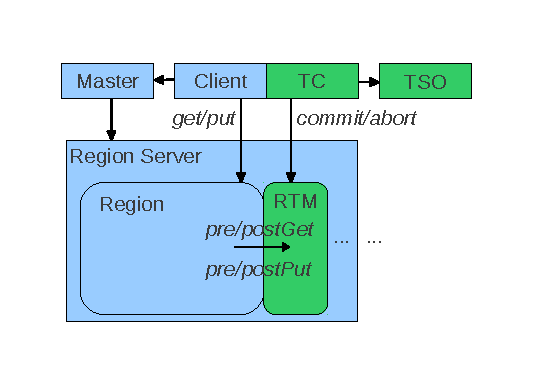
\includegraphics{images/tm.pdf}
\caption{Transaction Manager}
\label{tm}
\end{figure}

\subsection{Region Transaction Manager}
The RTM implements the MVTO protocol for all rows in the region it is associated with. It does this by intercepting all read and write operations through the region observer coprocessor interface. It also acts as a coprocessor endpoint to expose local commit and abort operations to TCs. The MVTO implementation at the core of the RTM is agnostic of the underlying datastore, i.e. although we apply it to HBase regions, any datastore that satisfies the underlying assumptions can make use of it.

\subsubsection{Writes}
The RTM is notified by the region whenever a row is about to be written and immediately after it was written. It processes the before-write notification by applying rule 2.a of the MVTO protocol for each column in the row touched by the write: If an older version of any column in the row has already been read by a younger transaction, then the current transaction is aborted. The RTM also remembers each cell written by the transaction so that it can remove them in case the transaction is aborted. Although the write itself is executed as an atomic unit, the notifications are not part of that unit. In particular, it is possible for a read operation to occur in between a write and one of the corresponding notifications. Therefore, the RTM also remembers which writes are currently in progress until it receives a notification that they have completed.

\subsubsection{Reads}
Read operations retrieve all versions in the row whose timestamp are smaller than that of the transaction. The result set is passed to the RTM as part of the post-read notification, so it can filter it based on rule 1. of the MVTO protocol. For each column in the row it traverses the versions in descending order and applies the following algorithm: if the current version was written by an aborted transaction, the version is removed from the result set and the next is tried. Otherwise, the RTM records that the transaction read this version and removes all older versions of this column from the result set. If the transaction that wrote the version is still active, the RTM also records a read-from relationship between the transactions, so it can delay the commit or cascade aborts as needed. Prior to iterating over the versions, the RTM also checks if a pending write for a newer version exists that should be part of the result set, but is not (because it has not been applied to the region yet). If this is the case, the reading or writing transaction must be aborted, because the reader has a view of the data that is inconsistent with the timestamp ordering. In other words, the read appears to have been scheduled before the write, however, if that were the case, the write would not have been admitted.

\subsubsection{Deletes}
Deletes are handled as a special case of writes. Clients write a null value and annotate the operation with a delete flag, which the RTM remembers when it is notified about the write. When data is read, any versions that are flagged as deleted are removed from the result set. After a transaction has committed, versions marked as deleted are permanently removed from the region, so they no longer need to be filtered out.

\subsubsection{Aborts and Commits}
When a transaction is aborted, the RTM no longer considers it during write conflict detection. After the abort has been recorded, the RTM asynchronously finalizes the transaction by aborting any transactions that read from it and deleting any versions it has written into the datastore, including delete markers. When a transaction commits, the RTM waits until all transactions it read from have committed before recording the commit. In the asynchronous commit finalizer it notifies transactions that read from the committed transaction about the commit and permanently applies deletes by removing delete markers and all older versions of the given cell in the datastore.

\subsubsection{Version Cleanup}
The operations described above only remove versions from the datastore that were written by aborted transactions or by delete operations of committed transactions. It is also necessary to remove committed versions that have been superseded by newer committed versions. While it would be possible to issue delete operations to the datastore as part of the post-commit finalizers, a more efficient approach is to hook a garbage collector into the region compaction process to simply omit old versions when new HFiles are written. This approach was developed in ~\cite{Junqueira:2011:LTS:2056318.2057148}. For this purpose, RTMs expose an operation that returns the oldest active transaction timestamp at any given time. For each cell, the garbage collector can omit any versions that carry timestamps smaller than that one, except for the last.

\subsubsection{Data Structures}
Each transaction is represented by an in-memory data structure that stores the state, the keys for read and written versions, and references to other transactions it read from. Three separate indices on these transactions are maintained in order to provide for efficient lookup and conflict detection. The main index is a binary search tree on the TID. It is used for direct lookup and to peridiodically scan transactions in the order they started to determine the first active transaction. In the processes any finalized aborted transaction is removed from the indices. Any finaliezd committed transaction that preecedes the first active transaction is also removed and garbage collected, but finaliezd committed transactions that follow it must be kept around, since they are still potentially needed for conflict detection. The second index stores transactions by the versions they have read by hashing keys (row+column) onto sorted maps of versions to sorted transaction sets. The third index is a hash map from keys to transactions that temporarily stores transactions by keys they are in the process of writing.

\subsubsection{Recovery}
RTMs must be able to survive region restarts, crashes, splits, and moves. Therefore, the data structures need to be recoverable from persistent storage. RTMs do this by logging each transaction operation to a write-ahead log, which is stored in a table by region. Old log entries are prediodically purged from the table based on the first active transaction timestamp. This reduces resource usage and speeds up the recovery process. When an RTM recovers from a region crash, it replays all log entries from its log into the data structures and then aborts transactions that were active at the time of the crash. Logging could be optimized using group commits ~\cite{Weikum:2001:TIS} on a per-region basis, but we leave this for future work.

\subsubsection{Distributed Transactions}
Although the main goal of this work is to provide means to localize transactions, we also need to support distributed transactions so that applications can initially run unoptimized and our learning algorithm can detect groupings. Users may also have a need for distributed transactions in production in certain situations where grouping is not possible. Distributed transactions are implemented via Zookeeper. When a TC detects the need for a distributed transaction, it creates a special transaction node in Zookeeper that identifies the transaction. Each RTM when asked to enlist in the distributed transaction creates an ephemeral sequence node under the transaction node. The RTM uses the node to vote for the outcome and the TC uses the node to detect server failure and to decide the outcome.

\subsection{Timestamp Oracle}
Globally unique timestamps are needed to ensure that the MVTO protocol generates globally serializable schedules. It would be possible to implement Lamport clocks ~\cite{Lamport:1978:TCO:359545.359563} for this purpose, but using a centralized timestamp server is an approach adopted by many recent distributed transaction managers that rely on timestamp ordering (e.g., ~\cite{Peng:2010:LIP:1924943.1924961, Wei:2011:5740834}). The TSO must be highly available and recoverable. To achieve this, it can use a similar fail-over mechanism to the HBase master, in which a hot-standby monitors Zookeeper to take over if the primary were to fail. The primary TSO either replicates the latest timestamp it has handed out or persists it in shared storage, so the secondary can resume to generate increasing timestamps. To reduce the number of RPCs or disk accesses, group commits can be applied here as well.

\subsection{Transaction Client}
The transaction management components described thus far can be used directly through the HBase API to implement transactions. However, to facilitate this task, we have implemented a client API wrapper around the HBase API. This TC is used to demarcate transaction boundaries using the familiar begin-commit-rollback idiom and it encapsulates the mapping of entity groups to regions to optimize for local transactions.

\subsubsection{API}
- closely resembles HBase API: API for creating tables and for creating/putting/deleting data.
- timestamps are not exposed in the API, because they are managed by the system
- additional API for defining entity groups across tables
- scanners currently not supported

\subsubsection{Entity Groups}


\subsubsection{Transaction Implementation}
- a transaction is initially started as a local transaction
- once an entity from a different entity group is accessed, the TC converts it into a distributed transaction
- note that the entity could be co-located in the same region, but the client 


\section{Entity Group Detection}


\section{Progress}
We have made significant progress on the transaction manager implementation. The main functionality of the RTM is in place and tested on HBase. We still need to complete the implementation of the recovery log, support fluent region splits, and add distributed transactions. We also need to finish the fail-over implementation of the TSO. On the TC side, we have the initial APIs in place, but need to implement entity groups in full generality.

In our entity group detection algorithm ...


\section{Methods}
To implement our proposal, we will utilize and build on several tools that are being developed in the context of the Apache Hadoop project. Specifically, we will harness the Hadoop Distributed File System (HDFS), the Hadoop database (HBase), and Zookeeper. We refer to these three components as the foundation. We will extend the foundation with four components which are combined to form a cohesive system: a transaction manager, an observer, an analyzer, and a partitioner. We will describe each component separately in the following subsections.

\subsection{Foundation}
The basis for the foundation is HDFS, a popular open source implementation of the Google File System (GFS) ~\cite{Ghemawat:2003:GFS:1165389.945450}. It has a master/slave architecture which consists of a central Namenode server that monitors the system and multiple DataNodes which actually contain the data. The NameNode contains all the metadata and responds to remote procedure calls(RPC) from clients and DataNodes. It is highly scalable in growing up to large clusters for applications which will need to process heavy workloads and has been utilized in clusters that contain thousands of nodes.  HDFS communication protocols operate at the Internet TCP/IP protocol making it ideal for web applications. Also, data integrity is assured as HDFS implements checksum verification on files. By computing the checksum on a transferred file and comparing it to the stored checksum, HDFS can ensure that no bits have been lost or misplaced during file transfer. If an inconsistency is detected, the file is marked as corrupted and the system may take the necessary steps to correct the error.  Data replication is also handled transparently, which makes HDFS fault tolerant with respect to transient failures in the nodes such as a server crash or a network outage. HDFS will automatically pair clients with the replica of the data nearest to it. This ensures the shortest possible transfer time to a user if an application is deployed across multiple datacenters on a wide area network. Since the Internet spans the entire globe, there can be significant improvements in accessing data from a local datacenter as opposed to waiting for data to travel thousands of miles to wait for a response. Files in HDFS are typically immutable, which simplifies many tasks such as replication, but also provide an append operation, which is particularly useful for writing transaction logs. Finally, it should be noted that HDFS is written in the Java programming language and also exposes Java APIs, which has several advantages, such as ease of development, broad community support, and portability. The inherent scalability, data replication, and consistency features provide a powerful abstraction that facilitates the task of building a distributed database.

On top of HDFS, we will run the HBase database which is one of the most popular NoSQL databases. It is an open source implementation of Google's BigTable ~\cite{Chang:2006:BDS:1267308.1267323} for storing structured data in a versioned, column-oriented table format. Tables are automatically sorted by row key, partitioned into row ranges (regions), and distributed across so called region servers. Region servers store regions in HDFS files in the form of indexed blocks to make them quickly accessible. Since HDFS files are immutable, any data updates are stored in memory and appended to a write-ahead log file using HDFS's append capability. Region servers run several compaction algorithms to periodically flush in-memory data by merging it with existing HDFS files and writing out consolidated HDFS files. Old HDFS files are removed in the process. This log and merge based approach can deliver substantial performance improvements compared to B-trees used in RDBMSs, because it avoids expensive disk seeks. Clients connect to region servers via a master server, which maintains the mapping from row ranges to region servers. They subsequently cache the information and only need to retrieve it again when the accessed row range is assigned to a different region server, which happens infrequently for a given row range. To increase the storage and processing capacity new region servers can be added to an existing cluster. This design makes HBase linearly scalable to large cluster sizes. HBase provides full ACID transactions for single row operations; modifications to multiple rows can be submitted in batch, but are not guaranteed to complete atomically. Like HDFS, HBase also has a Java API to allow application developers to interface with it.  It also supports a variety of other APIs like Thrift and Rest for non-Java developers.

The final foundation component we expect to utilize is Apache Zookeeper, which is already used by HBase for several configuration functions, such as monitoring availability of region servers. Zookeeper ~\cite{Hunt:2010:ZWC:1855840.1855851} is an open source project that implements a modified version of the Paxos algorithm ~\cite{Lamport:1998:PP:279227.279229, Lamport:2001:PMS} to facilitate coordination among distributed applications. It exposes a hierarchical namespace similar to a file system interface which provides atomic and conditional writes, notifications, and ephemeral nodes as primitives for building higher-level distributed coordination services. It's lock free nature makes it well suited for implementing scalable distributed transaction management.

\subsection{Transaction Manager}
We plan to build a distributed transaction management layer on top of HBase that provides full ACID guarantees within partitions and also supports distributed transactions across partitions. HBase was recently enhanced with basic building blocks for supporting multi-row transactions for co-located data, which we plan to leverage. To enable distributed transactions we plan to use Zookeeper for reaching consensus on log writes and commits. Isolation will be guaranteed using multiversion concurrency control based on timestamp information built into the HBase data model. Our design is mainly inspired by Megastore, but we may also incorporate certain aspects of the CloudTPS design. In particular, the design approach of performing transactions on a consistent and replicated main memory cache seems promising and could likely benefit from a optimized partitioning scheme to co-locate data for fast access. The transaction management layer will provide a hook for observing the transaction log.

\subsection{Observer}
The observer collects any information needed to effectively analyze access patterns, data dependencies, and resource utilization. At a minimum this includes the transaction log entires observed via the transaction manager hook. It may also include metadata about requests such as client location, size of data, or access time. The status of cluster resources is relevant for data placement and must therefore also be collected. It consists of the current cluster topology, hardware information, such as memory size, hard disk size, and CPU speed, and resource utilization. To gather these data, the observer will use foundation APIs. Where necessary, additional hooks will be added to the foundation to expose relevant data. The observer feeds collected information into the analyzer.

\subsection{Analyzer}
The analyzer determines how data should be partitioned and where the formed partitions should be placed. We envision using a data warehouse to implement this component. The data warehouse could run on the same infrastructure to maximize utilization, or in a separate cluster to free the OLTP system from carrying the computational load. As such, possible implementation technologies include Apache Hive or a relational database system optimized for online analytical processing (OLAP). The data structures of this component will be optimized to run complex graph algorithms, clustering, and Markov chaining.

Graph theory has led to a variety of useful algorithms and concepts that should come in handy for the database partitioning problem.  Most graph partitioning problems are NP-hard so there are heuristic solutions available which can generate the appropriate node topology.  For example the Kernighan-Lin algorithm partitions two disjoint subsets so that the weight of the edges between them is minimized.  This is a technique which has traditionally been used in digital circuits, but may have uses in database partitioning.  Hypergraph theory is another promising idea in which one edge can connect to multiple vertices.  This type of a structure may be useful in simulating a distributed database topology where one network link may connect to a region with multiple nodes.  The Max-flow min-cut theorem is also useful in determining the weak cuts in a network that could cause the system to crash.  By using this theorem one could create more fault tolerant data centers in which there are few weak points that could stop important traffic in a system.

Clustering is another popular technique used in the field of machine learning to arrange similar data items together.  A specific form of clustering called hierarchical clustering involves minimizing the distance between related data items.  This would be useful in the database setting to minimize the network delay that a packet of data may experience traveling from one node to the next.  It would be especially useful in datacenters that span a wide area network where distance is indeed a major problem.  Centroid-based clustering is also useful because it finds the point within a cluster that has the shortest total distance to the other nodes.  This can be useful in determining where to place the central master node which has to communicate with all the nodes in its region.  A more general extension to this theory would involve Voronoi diagrams which arranges a diagram into multiple cells such that points in a cell are closer to each other than they are to points in other cells.

Markov chains are random processes which transition from one state to the next without retaining memory.  If we model Internet behavior as stochastic processes perhaps we may be better able to predict which data item a user may request to access next.  In this way, we may be able to improve the performance of databases by prefetching data items before they are requested.  This way, the user would not have to wait for data to travel from one server node to the next.  Google uses Markov chains for its PageRank algorithm to predict which websites a user will be most interested in visiting next given their current location ~\cite{Page_1998}.  Markov chains have also been used in queuing theory for networks to model the flow of incoming packets ~\cite{Bose02}.

\subsection{Partitioner}
The partitioner receives the output of the analysis phase and applies the determined partitioning scheme to the system while it is running. This may involve moving data items within partitions, repartitioning data, or moving partitions between servers. The critical requirement on the partitioner is to maintain strong consistency guarantees and minimize downtime while applying the partitions. We may be able to adapt some recently published approaches on live migration for RDBMS ~\cite{Das:2011:ALE:2002974.2002977, Elmore:2011:ZLM:1989323.1989356} to apply in the context HBase.

Overall, the goal of the architecture is to create modular components with minimal dependencies in order to maximize their generality and thus reusability. The observer, analyzer, and partitioner form a cycle that runs continuously and gives our system its self-managing character.

\section{Expected Results}
We expect to implement an extension of HBase that enhances its transaction processing capabilities while maintaining its high scalability. Furthermore, we will improve the performance of OLTP workloads through effective data partitioning and placement. In the process we will learn how to use and extend HDFS, HBase, and Zookeeper. We plan to evaluate our solution using one of the public workload benchmarks and compare the performance with other designs. As part of this evaluation we will consider different workloads and failure cases to identify the strengths and weaknesses of our proposed design.

% Bibliography generation from references.bib
\bibliographystyle{IEEEtran}
\bibliography{IEEEabrv,references}

\end{document}
